% DOCUMENT TYPE: PRESENTATION
\documentclass[12pt]{beamer}

% PACKAGES TO USE
\usepackage[utf8]{inputenc}
\usepackage[spanish]{babel}
\usepackage{lastpage}
\usepackage{subcaption}
\usepackage[export]{adjustbox}

% CONFIGURATIONS
\setbeamertemplate{footline}[frame number]

% PRESENTATION INFO
\title{Reconstrucción de Huellas Dactilares Digitales Utilizando un Modelo Generativo Adversarial Convolucional}
\author{Cristian Yesid Andrade Hernández}
\institute{Universidad de los Andes}
\date{2020}

% DOCUMENT
\begin{document}

% ==== INIT SLIDE ====
\frame[plain]{\titlepage}

% ==== SLIDE 2 ====
\begin{frame}{Introducción}

    Captura digital de impresión dactilar del dedo índice.

    \begin{figure}[h]
        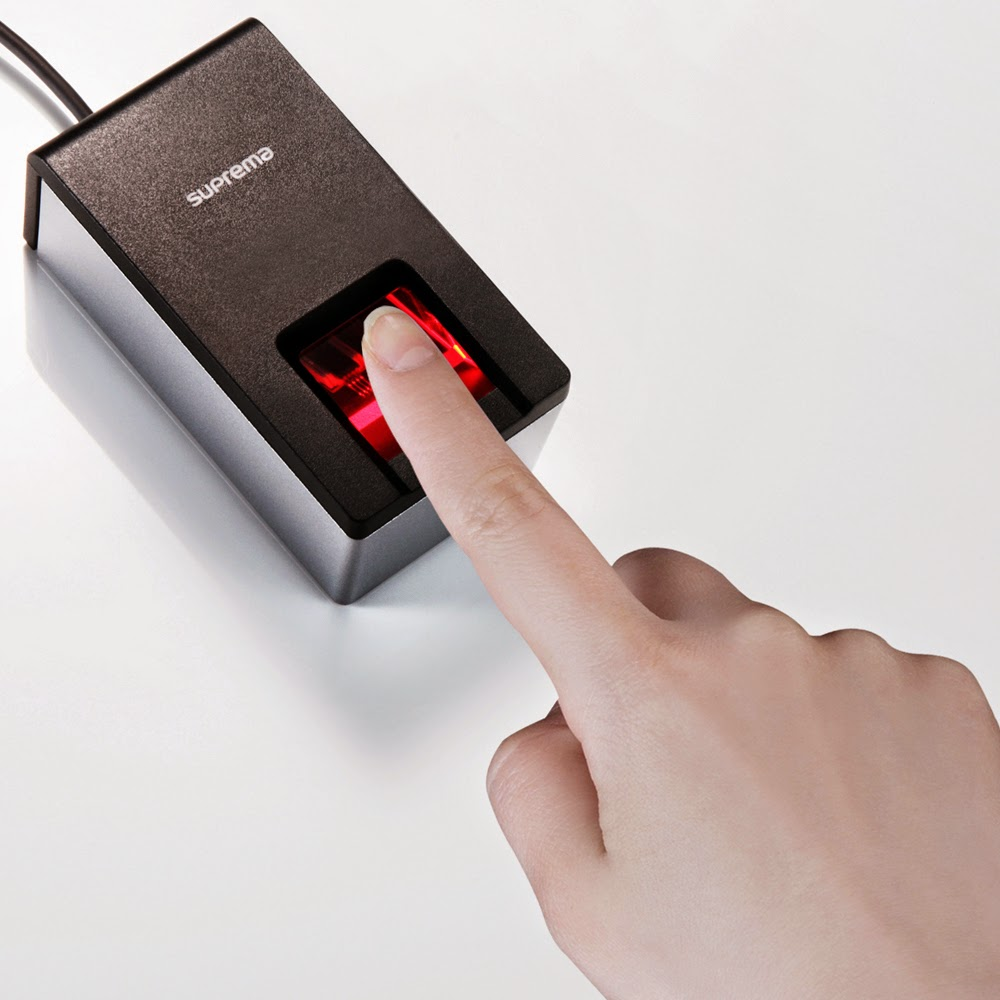
\includegraphics[scale=0.15]{figs/dedo_lector_biometrico.jpg}
        \caption{Lector Biométrico Óptico}
    \end{figure}
    
\end{frame}

% ==== SLIDE 3 ====
\begin{frame}{Introducción}

    Huellas dactilares digitalizadas con alguna condición de deterioro o modificación.
    \vspace{5mm}

    \begin{figure}[h]
        \begin{subfigure}{0.45\textwidth}
            \centering
            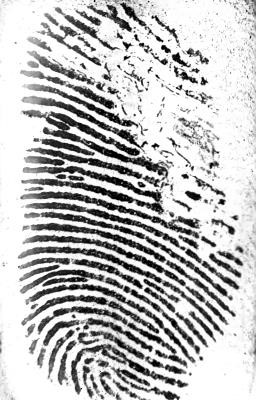
\includegraphics[scale=0.4]{figs/deteriorada_1.jpg}  
            \caption{Huella Borrosa}
        \end{subfigure}
        \begin{subfigure}{0.45\textwidth}
            \centering
            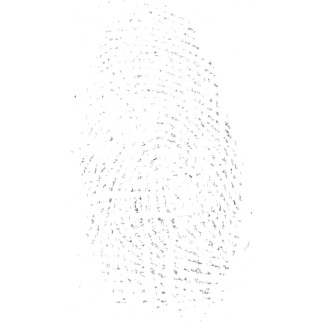
\includegraphics[scale=0.42]{figs/deteriorada_0.png}  
            \caption{Huella Incompleta}
        \end{subfigure}
    \end{figure}

\end{frame}

% ==== SLIDE 4 ====
\begin{frame}{Introducción}

    \begin{figure}[h]
        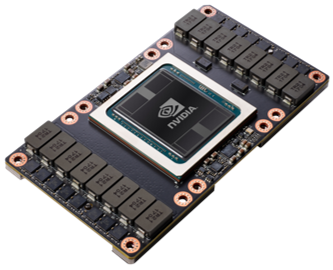
\includegraphics[scale=0.3]{figs/nvidia_card.png}
        \caption{Capacidad de Cómputo: GPU}
    \end{figure}
    
    \begin{figure}[h]
        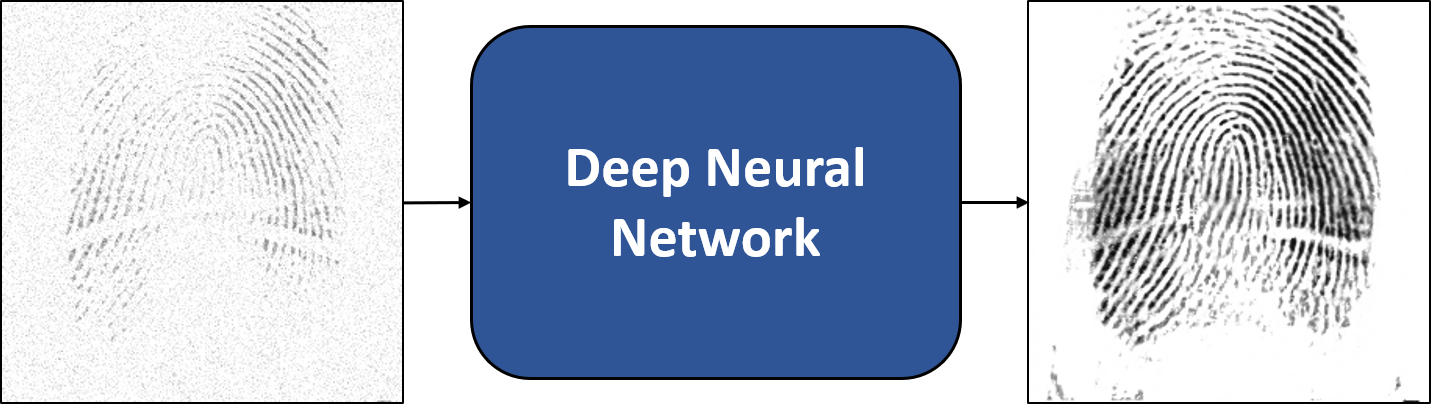
\includegraphics[scale=0.3]{figs/end_to_end.png}
        \caption{Modelo end to end}
    \end{figure}

\end{frame}

% ==== SLIDE 5 ====
\begin{frame}{Red Neuronal Convolucional}

    Composición de imagen digital de un canal.

    \begin{figure}[h]
        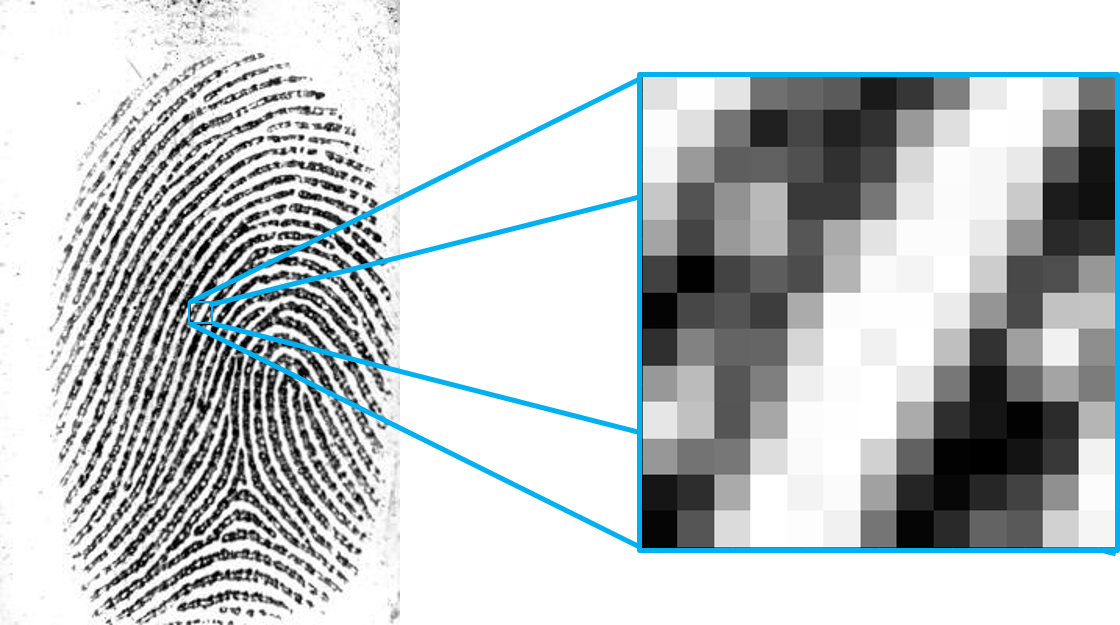
\includegraphics[scale=0.45]{figs/huella_pixeles.png}
        \caption{Huella Dactilar Digital}
    \end{figure}

\end{frame}

% ==== SLIDE 6 ====
\begin{frame}{Red Neuronal Convolucional}

    Lógica de la operación de convolución y convolución transpuesta en dos dimensiones aplicada a una imagen.

    \begin{figure}[h]
        \begin{subfigure}{0.45\textwidth}
            \centering
            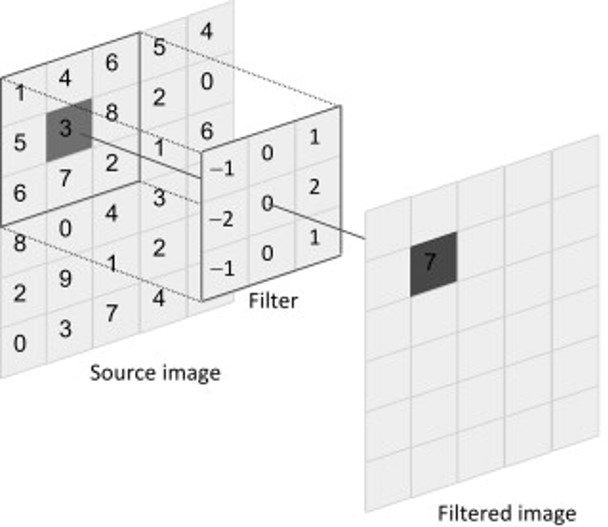
\includegraphics[scale=0.325]{figs/conv_2d.jpg}  
            \caption{Convolución}
        \end{subfigure}
        \begin{subfigure}{0.45\textwidth}
            \centering
            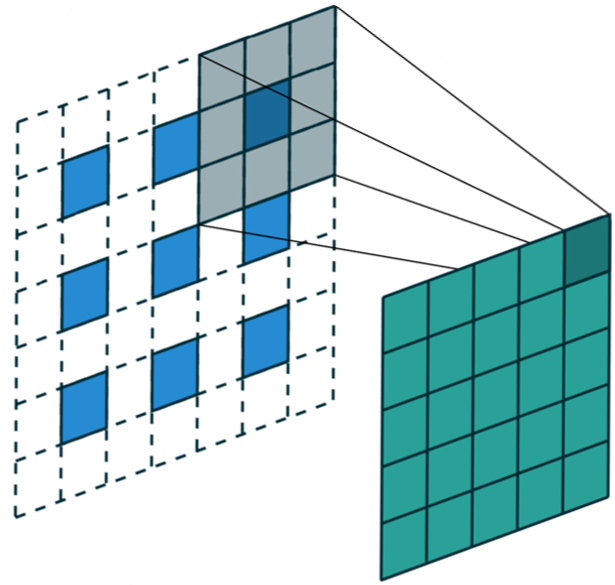
\includegraphics[scale=0.30]{figs/trans_conv.PNG}  
            \caption{Convolución Transpuesta}
        \end{subfigure}
    \end{figure}

\end{frame}

% ==== SLIDE 7 ====
\begin{frame}{Red Neuronal Convolucional}

    Ventajas de usar un modelo de capas convolucionales:
    \vspace{5mm}
    
    \begin{itemize}
        \item Características de bajo y alto nivel que se utilizan en la reconstrucción.
        \vspace{4mm}
        
        \begin{figure}[h]
            \begin{subfigure}{0.18\textwidth}
                \centering
                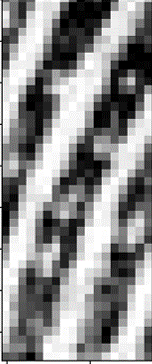
\includegraphics[scale=0.16]{figs/fll_0.png}  
                \caption{Cresta Vertical}
            \end{subfigure}
            \begin{subfigure}{0.18\textwidth}
                \centering
                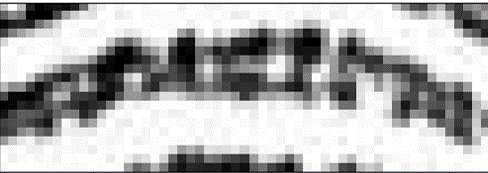
\includegraphics[scale=0.16]{figs/fll_1.png}  
                \caption{Cresta Horizontal}
            \end{subfigure}
            \begin{subfigure}{0.18\textwidth}
                \centering
                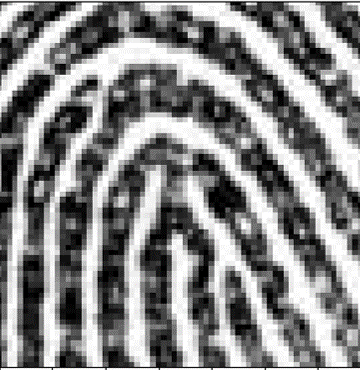
\includegraphics[scale=0.16]{figs/fhl_0.png}  
                \caption{Núcleo}
            \end{subfigure}
            \begin{subfigure}{0.18\textwidth}
                \centering
                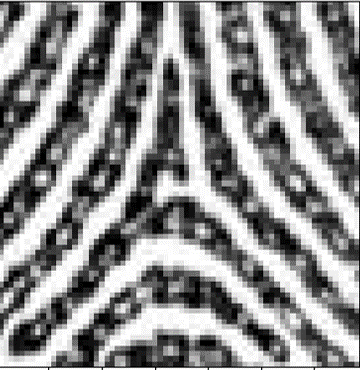
\includegraphics[scale=0.16]{figs/fhl_1.png}  
                \caption{Delta}
            \end{subfigure}
        \end{figure}
        
        \vspace{3mm}
        
        \item Modelo convolucional: 15 millones de parámetros. Perceptrón multicapa: 1000 millones de parámetros
        
    \end{itemize}

\end{frame}

% ==== SLIDE 8 ====
\begin{frame}{Red Neuronal Convolucional}

    Modelo convolucional de reconstrucción y mejora de impresiones dactilares digitales.

    \begin{figure}[h]
        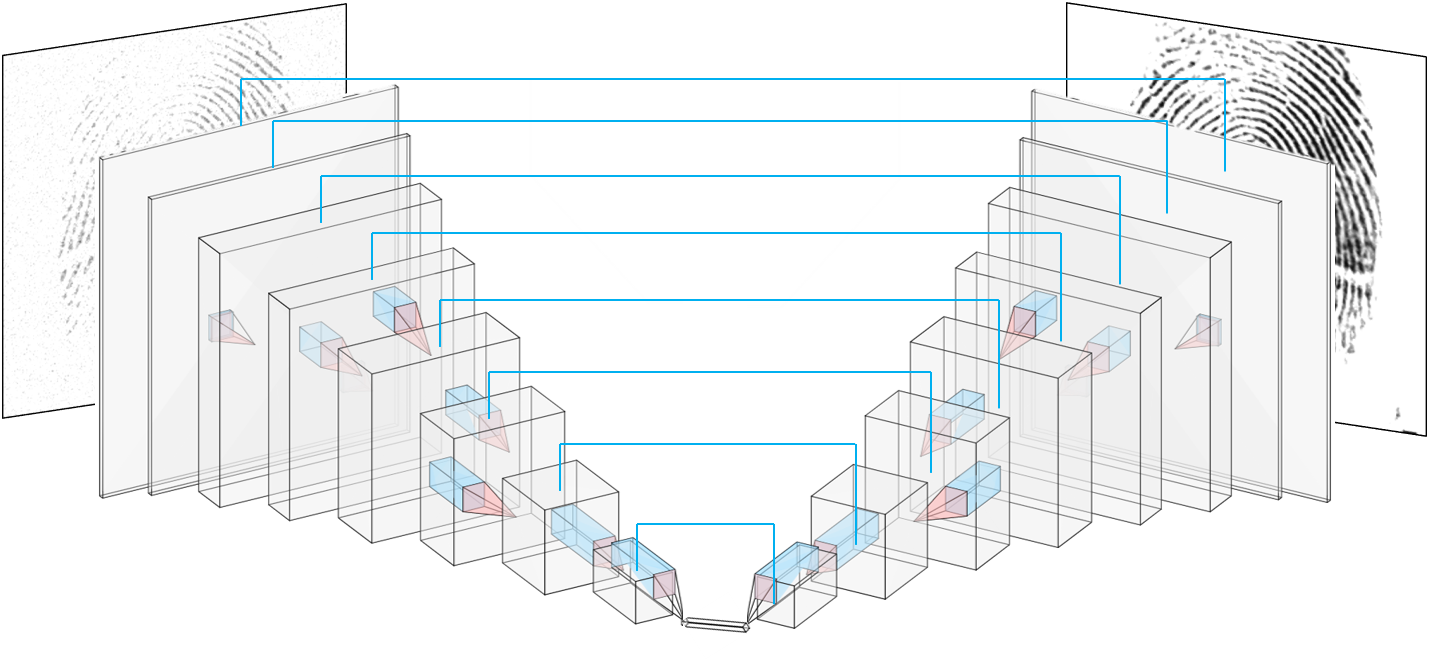
\includegraphics[scale=0.42]{figs/layers_nn_u.PNG}
        \caption{Autoencoder en Configuración U-Net (Generador)}
    \end{figure}

\end{frame}


% ==== SLIDE 9 ====
\begin{frame}{Red Neuronal Convolucional}

    \begin{figure}[h]
        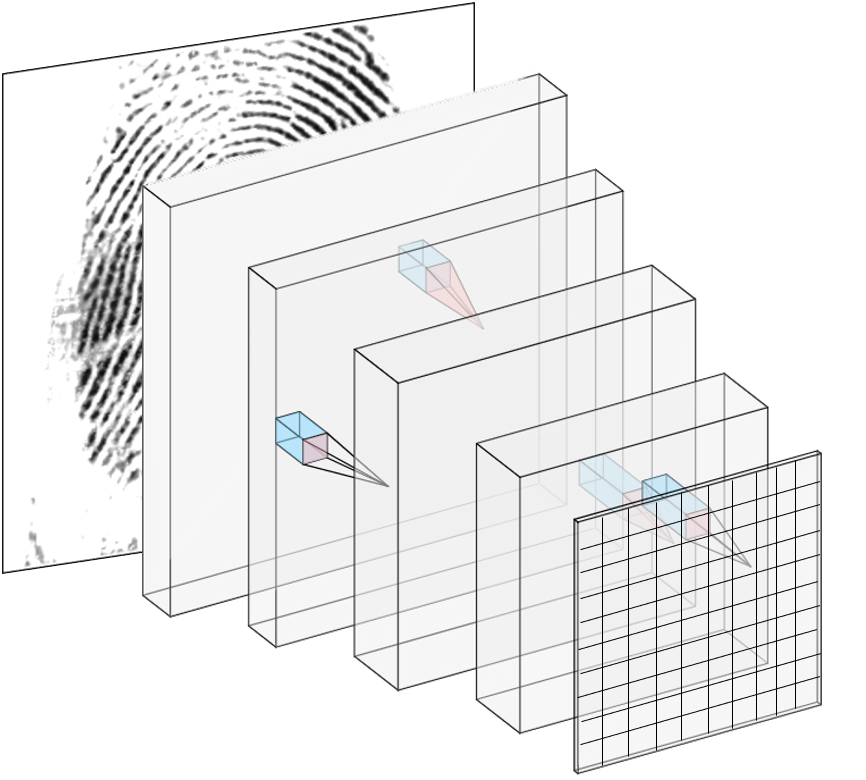
\includegraphics[scale=0.4]{figs/disc_cuad.png}
        \caption{Encoder en configuración PATCH (Discriminador)}
    \end{figure}

\end{frame}

% ==== SLIDE 10 ====
\begin{frame}{Entrenamiento del modelo}

    \begin{figure}[h]
        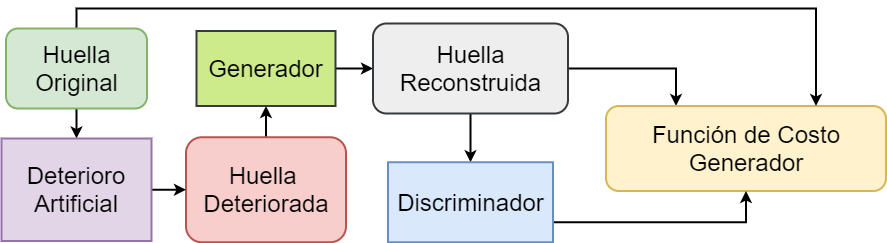
\includegraphics[scale=0.27]{figs/training_flow_gen.png}
        \caption{Cálculo de Costo del Generador}
    \end{figure}
    \vspace*{-5mm}
    \begin{figure}[h]
        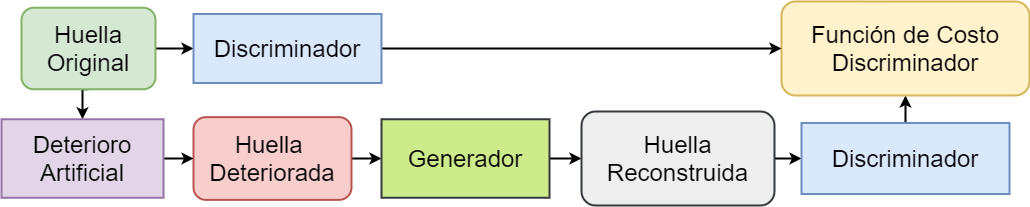
\includegraphics[scale=0.27]{figs/training_flow_disc.png}
        \caption{Cálculo de Costo del Discriminador}
    \end{figure}

\end{frame}

% ==== SLIDE 11 ====
\begin{frame}{Entrenamiento del modelo}

     Función de costo asociada al generador del modelo.
    \begin{equation}
        Gen_{loss} = \alpha||y-gen(x)||_{[1]} - log(disc(x,gen(x)))
    \end{equation}
    Función de costo asociada al discriminador del modelo.
    \begin{equation}
        Disc_{loss} = -log(1-disc(x,gen(x)))-log(disc(x,y))
    \end{equation}
    
    El parámetro \textit{y} corresponde a la huella original, \textit{x} a la huella deteriorada y $\alpha$ define el peso del componente reconstructivo en la expresión.

\end{frame}

% ==== SLIDE 12 ====
\begin{frame}{Entrenamiento del modelo}

    {\scriptsize
    El modelo se implementó utilizando el framework TensorFlow soportado en Python.

    \begin{figure}[h]
        \begin{subfigure}{0.4\textwidth}
            \centering
            
\includegraphics[scale=0.2]{figs/tensorflow.png}
        \end{subfigure}
        \begin{subfigure}{0.46\textwidth}
            \centering
            
\includegraphics[scale=0.03]{figs/python.png}  
        \end{subfigure}
    \end{figure}
    
     Configuración del algoritmo de entrenamiento:
     
     \begin{itemize}
        \item Batch size: 48
        \item Optimizador: ADAM.
        \item Beta 1: 0.5
        \item Beta 2: 0.999
        \item Tasa de aprendizaje: 0.00018
        \item $\alpha:$ 40
        \item Épocas: 96
    \end{itemize}
    
    Se utilizó la unidad de procesamiento gráfico NVIDIA Tesla K40 disponible el cluster de cómputo de la Universidad de los Andes.
    }
    
\end{frame}

% ==== SLIDE 13 ====
\begin{frame}{Resultados}

    \begin{figure}[h]
        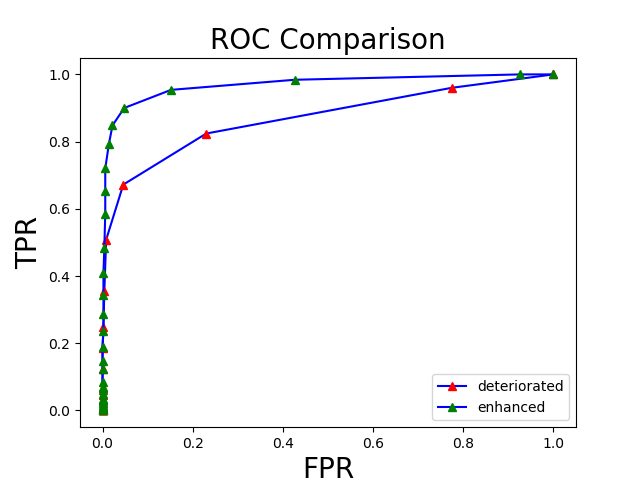
\includegraphics[scale=0.56]{figs/roc_comparison.png}
        \caption{Receiver Operating Characteristic}
    \end{figure}
    
\end{frame}

% ==== SLIDE 14 ====
\begin{frame}{Resultados}

    \begin{figure}[h]
        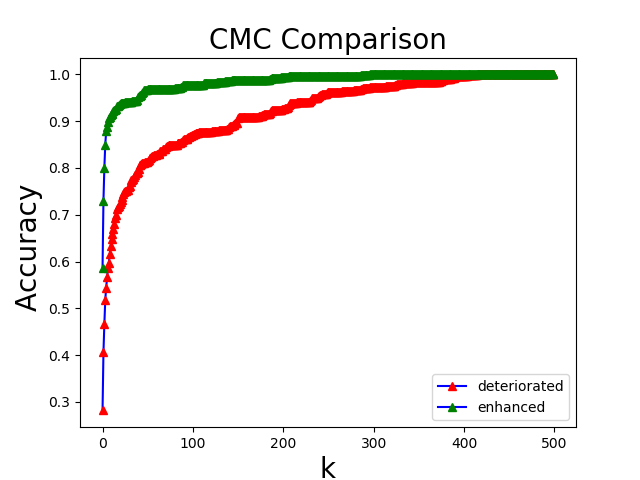
\includegraphics[scale=0.56]{figs/cmc_comparison.png}
        \caption{Cummulative Match Curve}
    \end{figure}
    
\end{frame}

% ==== SLIDE 15 ====
\begin{frame}{Resultados}

    \begin{figure}[h]
        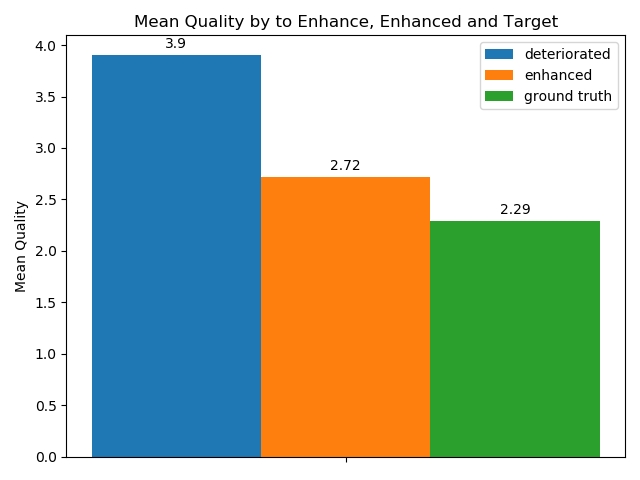
\includegraphics[scale=0.56]{figs/mean_qualities.png}
        \caption{Medida de Calidad de las Huellas}
    \end{figure}
    
\end{frame}

% ==== SLIDE 16 ====
\begin{frame}{Referencias}

{\tiny
[1] C. Watson, M. Garris, E.T.C.W.R.M.S.J.K.K., 2007. User’s Guide to
NIST Biometric Image Software. National Institute of Standards and
Technology.\\
[2] D. Maltoni, D. Maio, A.J., Prabhakar, S., 2009. Handbook of fingerprint recognition. Springer Science+Business Media.\\
[3] NIST, 2019. Nist biometric image software (nbis).
URL: https://www.nist.gov/services-resources/software/nist-biometric-image-software-nbis.\\
[4] O. Ronneberger, P. Fischer, T.B., 2015. U-net: Convolutional networks
for biomedical image segmentation. Computer Science Department and BIOSS Centre for Biological Signalling Studies, University of Freiburg, Germany.\\
[5] P. Isola, J. Zhu, T.Z.A.E., 2016. Image-to-image translation with conditional adversarial networks arXiv:arXiv:1611.07004.\\
[6] R.M. Bolle, J.H. Connell, S.P.N.R., Senior, A., 2005. The relation between the roc curve and the cmc, in: In Proc: Fourth IEEE Workshop on Automatic Identification Advanced Technologies Conference, Buffalo,
NY, USA.
}
    
\end{frame}

\end{document}

%command	8pt	9pt	10pt	11pt	12pt	14pt	17pt	20pt
%tiny	5pt	5pt	5pt	6pt	6pt	6pt	8pt	10pt
%scriptsize	5pt	6pt	7pt	8pt	8pt	8pt	10pt	12pt
%footnotesize	6pt	7pt	8pt	9pt	10pt	10pt	12pt	14pt
%small	7pt	8pt	9pt	10pt	11pt	12pt	14pt	17pt
%normalsize	8pt	9pt	10pt	11pt	12pt	14pt	17pt	20pt
%large	10pt	10pt	12pt	12pt	14pt	17pt	20pt	25pt
%Large	11pt	11pt	14pt	14pt	17pt	20pt	25pt	29.86pt
%LARGE	12pt	12pt	17pt	17pt	20pt	25pt	29.86pt	35.83pt
%huge	14pt	14pt	20pt	20pt	25pt	29.86pt	35.83pt	42.99pt
%Huge	17pt	17pt	25pt	25pt	25pt	35.83pt	42.99pt	51.59pt